\documentclass[11pt]{exam}

\usepackage{amssymb, amsmath, amsthm, mathrsfs, multicol, graphicx} 
\usepackage{tikz}

\def\d{\displaystyle}
\def\?{\reflectbox{?}}
\def\b#1{\mathbf{#1}}
\def\f#1{\mathfrak #1}
\def\c#1{\mathcal #1}
\def\s#1{\mathscr #1}
\def\r#1{\mathrm{#1}}
\def\N{\mathbb N}
\def\Z{\mathbb Z}
\def\Q{\mathbb Q}
\def\R{\mathbb R}
\def\C{\mathbb C}
\def\F{\mathbb F}
\def\A{\mathbb A}
\def\X{\mathbb X}
\def\E{\mathbb E}
\def\O{\mathbb O}
\def\pow{\mathscr P}
\def\inv{^{-1}}
\def\nrml{\triangleleft}
\def\st{:}
\def\~{\widetilde}
\def\rem{\mathcal R}
\def\iff{\leftrightarrow}
\def\Iff{\Leftrightarrow}
\def\and{\wedge}
\def\And{\bigwedge}
\def\AAnd{\d\bigwedge\mkern-18mu\bigwedge}
\def\Vee{\bigvee}
\def\VVee{\d\Vee\mkern-18mu\Vee}
\def\imp{\rightarrow}
\def\Imp{\Rightarrow}
\def\Fi{\Leftarrow}

\def\={\equiv}
\def\var{\mbox{var}}
\def\mod{\mbox{Mod}}
\def\Th{\mbox{Th}}
\def\sat{\mbox{Sat}}
\def\con{\mbox{Con}}
\def\bmodels{=\joinrel\mathrel|}
\def\iffmodels{\bmodels\models}
\def\dbland{\bigwedge \!\!\bigwedge}
\def\dom{\mbox{dom}}
\def\rng{\mbox{range}}
\DeclareMathOperator{\wgt}{wgt}

\def\circleA{(-.5,0) circle (1)}
\def\circleAlabel{(-1.5,.6) node[above]{$A$}}
\def\circleB{(.5,0) circle (1)}
\def\circleBlabel{(1.5,.6) node[above]{$B$}}
\def\circleC{(0,-1) circle (1)}
\def\circleClabel{(.5,-2) node[right]{$C$}}
\def\twosetbox{(-2,-1.5) rectangle (2,1.5)}
\def\threesetbox{(-2,-2.5) rectangle (2,1.5)}


\def\bar{\overline}

%\pointname{pts}
\pointsinmargin
\marginpointname{pts}
\addpoints
\pagestyle{head}
\printanswers

\firstpageheader{Math 228}{\bf Homework 3 Solutions}{Feb 8, 2012}


\begin{document}




\begin{questions}
\question[4] In a recent survey, 30 students reported whether they liked their potatoes Mashed, French-fried, or Twice-baked. 15 liked them mashed, 20 liked French fries, and 9 liked twice baked potatoes. Additionally, 12 students liked both mashed and fried potatoes, 5 liked French fries and twice baked potatoes, 6 liked mashed and baked, and 3 liked all three styles. How many students
{\em hate} potatoes?  Explain why your answer is correct.

\begin{solution}
  Using the principle of inclusion/exclusion, the number of students who like their potatoes in at least one of the ways described is \[15 + 20 + 9 - 12 - 5 - 6 + 3 = 24.\]  Therefore there are $30-24 = 6$ students who do not like potatoes.  You can also do this problem with a Venn diagram.
\end{solution}

\question[6] Consider the set $S = \bar A \cup (B \cap \bar C)$.
\begin{parts}
  \part Draw a Venn diagram for the set $S$.
  \begin{solution}
    \begin{center}
      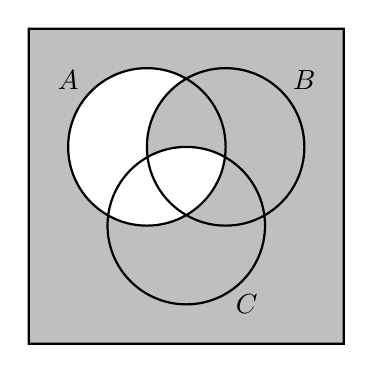
\begin{tikzpicture}[fill=gray!50]
      \fill \threesetbox;
\begin{scope}
  \clip \threesetbox \circleB;
  \fill[white] \circleA;
\end{scope}
\begin{scope}
  \clip \circleC;
  \fill[white] \circleA;
\end{scope}

\draw[thick] \circleA \circleAlabel \circleB \circleBlabel \circleC \circleClabel \threesetbox;
\end{tikzpicture}
    \end{center}

  \end{solution}

  \part Use the Venn diagram from part (a) to draw a Venn diagram for $\bar S$.
  
    \begin{solution}
    \begin{center}
      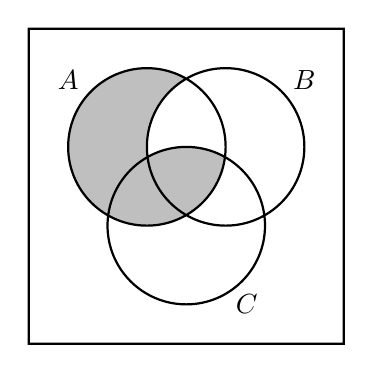
\begin{tikzpicture}[fill=gray!50]
\begin{scope}
  \clip \threesetbox \circleB;
  \fill \circleA;
\end{scope}
\begin{scope}
  \clip \circleC;
  \fill \circleA;
\end{scope}

\draw[thick] \circleA \circleAlabel \circleB \circleBlabel \circleC \circleClabel \threesetbox;
\end{tikzpicture}
    \end{center}

  \end{solution}
  \part Use the Venn diagram from part (b) to express $\bar S$ in terms for $A$, $B$ and $C$.  Your answer should have bars only over single letters.
  \begin{solution}
    $A \cap (\bar B \cup C)$
  \end{solution}

\end{parts}

\question[4] Let $A$, $B$, and $C$ be sets.  Suppose $A \subseteq B$ and $B \subseteq C$.  Does this mean $A \subseteq C$?  Explain why or why not. 

\begin{solution}
  Yes.  Let $x \in A$.  Since $A \subseteq B$, we know then that $x \in B$.  since $B \subseteq C$ then $x \in C$.  So every element of $A$ is also an element of $C$, which is just to say $A \subseteq C$.
\end{solution}


\question[6] Consider the function $f:\Z \to \Z$ defined by $f(n) = 2n + 3$.  
\begin{parts}
  \part Is $f$ one-to-one?  Explain.
  \begin{solution}
    $f$ is one-to-one.  Let $x$ and $y$ be integers, and suppose $f(x) = f(y)$.  So $2x + 3 = 2y+3$, which implies that $2x = 2y$ and as such $x = y$.  Thus the only way to get the same output is to start with the same input, which is to say $f$ is one-to-one.
  \end{solution}

  \part Is $f$ onto?  Explain.
  \begin{solution}
    $f$ is not onto.  For example, the integer $2$ in the codomain is not in the range, as the output of $f$ is always odd.
  \end{solution}

  \part Let $g: \R \to \R$ be defined by $g(x) = 2x + 3$.  Is $g$ onto?  Explain.
  \begin{solution}
    $g$ is onto (even though the rule defining $g$ is the same as the one for $f$ and $f$ is not onto).  Let $y \in \R$ be an element of the codomain.  We must find a value $x$ in the domain such that $2x + 3 = y$.  Take $x = \frac{y-3}{2}$.  This is a real number, so in the domain.  Of course, $2(\frac{y-3}{2}) + 3 = y$ so this $x$ works.  Since every real number is in the range, $g$ is onto.  
  \end{solution}

\end{parts}


\end{questions}




\end{document}


